\documentclass[a4paper,10pt]{article}
\usepackage[brazilian]{babel}
\usepackage[left=2.5cm,right=2.5cm,top=3cm,bottom=2.5cm]{geometry}
\usepackage{mathtools}
\usepackage{amsthm}
\usepackage{amsmath}
%\usepackage{nccmath}
\usepackage{amssymb}
\usepackage{amsfonts}
\usepackage{physics}
%\usepackage{dsfont}
%\usepackage{mathrsfs}

\usepackage{titling}
\usepackage{indentfirst}

\usepackage{bm}
\usepackage[dvipsnames]{xcolor}
\usepackage{cancel}

\usepackage{xurl}
\usepackage[colorlinks=true]{hyperref}

\usepackage{float}
\usepackage{graphicx}
%\usepackage{tikz}
\usepackage{caption}
\usepackage{subcaption}

%%%%%%%%%%%%%%%%%%%%%%%%%%%%%%%%%%%%%%%%%%%%%%%%%%%

\newcommand{\eps}{\epsilon}
\newcommand{\vphi}{\varphi}
\newcommand{\cte}{\text{cte}}

\newcommand{\N}{\mathbb{N}}
\newcommand{\Z}{\mathbb{Z}}
\newcommand{\Q}{\mathbb{Q}}
\newcommand{\R}{\vb{R}}
\newcommand{\C}{\mathbb{C}}
\renewcommand{\S}{\hat{S}}
%\renewcommand{\H}{\s{H}}

\renewcommand{\a}{\vb{a}}
\newcommand{\nn}{\hat{n}}
\renewcommand{\d}{\dagger}
\newcommand{\up}{\uparrow}
\newcommand{\down}{\downarrow}

\newcommand{\0}{\vb{0}}
%\newcommand{\1}{\mathds{1}}
\newcommand{\E}{\vb{E}}
\newcommand{\B}{\vb{B}}
\renewcommand{\v}{\vb{v}}
\renewcommand{\r}{\vb{r}}
\renewcommand{\k}{\vb{k}}
\newcommand{\p}{\vb{p}}
\newcommand{\q}{\vb{q}}
\newcommand{\F}{\vb{F}}

\newcommand{\s}{\sigma}
%\newcommand{\prodint}[2]{\left\langle #1 , #2 \right\rangle}
\newcommand{\cc}[1]{\overline{#1}}
\newcommand{\Eval}[3]{\eval{\left( #1 \right)}_{#2}^{#3}}

\newcommand{\unit}[1]{\; \mathrm{#1}}

\newcommand{\n}{\medskip}
\newcommand{\e}{\quad \mathrm{e} \quad}
\newcommand{\ou}{\quad \mathrm{ou} \quad}
\newcommand{\virg}{\, , \;}
\newcommand{\ptodo}{\forall \,}
\renewcommand{\implies}{\; \Rightarrow \;}
%\newcommand{\eqname}[1]{\tag*{#1}} % Tag equation with name

\setlength{\droptitle}{-7em}

\theoremstyle{plain}
\newtheorem{theorem}{Teorema}[section]
%\newtheorem{defi}[theorem]{Definição}
\newtheorem{lemma}[theorem]{Lema}
%\newtheorem{corol}[theorem]{Corolário}
%\newtheorem{prop}[theorem]{Proposição}
%\newtheorem{example}{Exemplo}
%
%\newtheorem{inneraxiom}{Axioma}
%\newenvironment{axioma}[1]
%  {\renewcommand\theinneraxiom{#1}\inneraxiom}
%  {\endinneraxiom}
%
%\newtheorem{innerpostulado}{Postulado}
%\newenvironment{postulado}[1]
%  {\renewcommand\theinnerpostulado{#1}\innerpostulado}
%  {\endinnerpostulado}
%
%\newtheorem{innerexercise}{Exercício}
%\newenvironment{exercise}[1]
%  {\renewcommand\theinnerexercise{#1}\innerexercise}
%  {\endinnerexercise}
%
%\newtheorem{innerthm}{Teorema}
%\newenvironment{teorema}[1]
%  {\renewcommand\theinnerthm{#1}\innerthm}
%  {\endinnerthm}
%
\newtheorem{innerlema}{Lema}
\newenvironment{lema}[1]
  {\renewcommand\theinnerlema{#1}\innerlema}
  {\endinnerlema}
%
%\theoremstyle{remark}
%\newtheorem*{hint}{Dica}
%\newtheorem*{notation}{Notação}
%\newtheorem*{obs}{Observação}


\title{\Huge{\textbf{Lista 1 - Estado Sólido 1}}}
\author{Mateus Marques}

\begin{document}

\maketitle

\section{}

(a) O gás de elétrons, em geral, é um sistema ideal composto de elétrons independentes (não interagem entre si) e livres (o potencial externo que age sobre eles é constante em todo ponto no interior do volume do sistema).

Podem ser feitas hipóteses adicionais sobre esse sistema. Se por exemplo houver interesse em calcular propriedades de transporte, pode-se supor que os elétrons entram em equilíbrio através de ``colisões instantâneas'' com um associado tempo de relaxação $\tau$, definido de maneira que a probabilidade de colisão por unidade de tempo seja $\tau^{-1}$.

\n

(b) No modelo de Drude consideramos apenas os elétrons de valência e são feitas as hipóteses adicionais descritas acima no item (a). Além disso também é suposto que as velocidades das partículas seguem a distribuição clássica de Boltzmann. Supondo um campo elétrico estacionário, utilizando a lei de Ohm ($\J = \sigma \E$) e a equação para o momento médio dos elétrons (obtida pela introdução do tempo de relaxação), obtém-se a fórmula de Drude para condutividade no regime estacionário:
$$
\sigma = \frac{ne^2\tau}{m_e}.
$$

\n

(c) As únicas diferenças do modelo semiclássico de Sommerfeld para o modelo clássico de Drude é a consideração dos elétrons como partículas quânticas (são descritos por funções de onda que satisfazem Schrödinger) que obedecem à estatística de férmions (distribuição de Fermi-Dirac, não mais obedecem à estatística de Boltzmann). As hipóteses do tempo de relaxação e do gás de elétrons são mantidas.

\n

(d) Sim, uma diferença importantíssima é que no modelo de Sommerfeld os elétrons obedecem ao princípio de exclusão de Pauli. Devido aos elétrons estarem confinados a um volume $V$ finito (mas mascroscópico), eles possuem momentos $\p = \hbar \k$ quantizados. Em condições periódicas, a quantização para o vetor quântico $\k$ é da forma $(k_x, k_y, k_z) = \qty(\frac{2\pi n_x}{L_x}, \frac{2\pi n_y}{L_y}, \frac{2\pi n_z}{L_z})$. Devido a $k$ ter unidade de inverso de comprimento, chamamos o espaço dos números ``$k$'' de espaço recíproco. Pelos elétrons serem férmions, o princípio de Pauli faz com que cada vetor quântico $\k$ consiga acomodar no máximo dois elétrons, um com spin up e outro com spin down.

\n

(e) Existem vários problemas, como a falta de dependência da temperatura no calor específico e condutividade, o modelo não conseguir exibir o comportamento em um campo elétrico AC ou num campo magnético. Mas eu acredito que o problema mais sério seja relacionado ao efeito Hall. Os dois modelos (Drude e Sommerfeld) prevêem um coeficiente Hall $R_H = - 1/ne$, que para alguns metais é bem diferente do previsto e para outros tem até o \textbf{sinal errado}, indicando portadores de carga positiva.

\section{}

(a) Simetria de translação é a invariância com respeito à translação, ou seja deslocamento por vetores $\r \to \r + \a$. Simetrias de translação só podem existir em sistema infinitos.

Simetria de ponto é uma invariância com respeito a realização de operações que estão atreladas em um único ponto, a saber as operações de rotação, reflexão, roto-reflexão e inversão. Simetrias de ponto podem ocorrer tanto em estruturas finitas (moléculas) como em estruturas infinitas (sistemas cristalinos).

\n

(b) Obs: Os vetores primitivos não são únicos, por isso usarei a expressão ``pode-se achar os vetores primitivos de tal forma'' no sentido de que eles existem na estrutura da rede, mas poderiam ser escolhidos outros vetores primitivos de qualidades diferentes.

\n

Os quatro grupos de simetria de rede para sistemas cristalinos 2D são:
\begin{itemize}
\item Rede quadrada: pode-se achar dois vetores primitivos ortonormais, ou seja, perpendiculares e de mesmo módulo. Exemplo $\a_1 = a \vu{x}$ e $\a_2 = a \vu{y}$.
\begin{figure}[H]
\centering
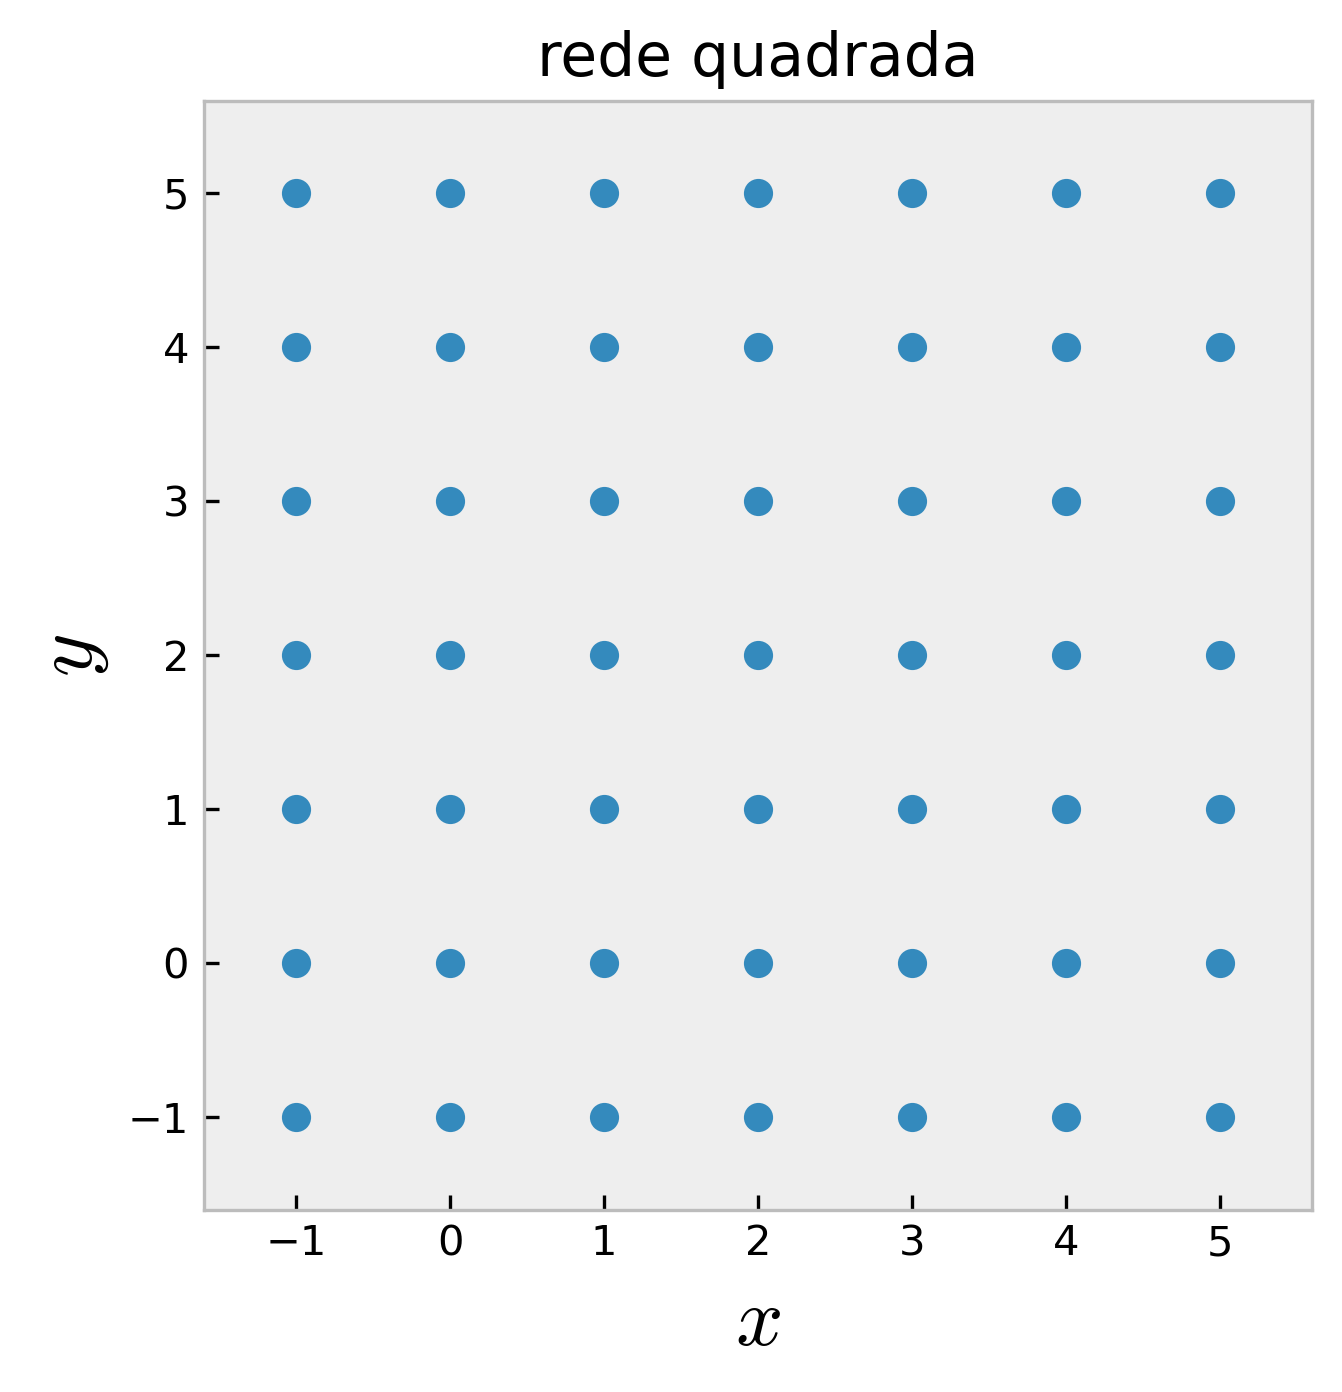
\includegraphics[width=0.35\linewidth]{fig/lattice_quad.png}
\caption{Rede Quadrada.}
\label{fig:lat-quad}
\end{figure}
\item Rede retangular: pode-se achar dois vetores primitivos ortogonais mas de módulo diferente. Exemplo: $\a_1 = a \vu{x}$ e $\a_2 = 1.5 a \,\vu{y}$.
\begin{figure}[H]
\centering
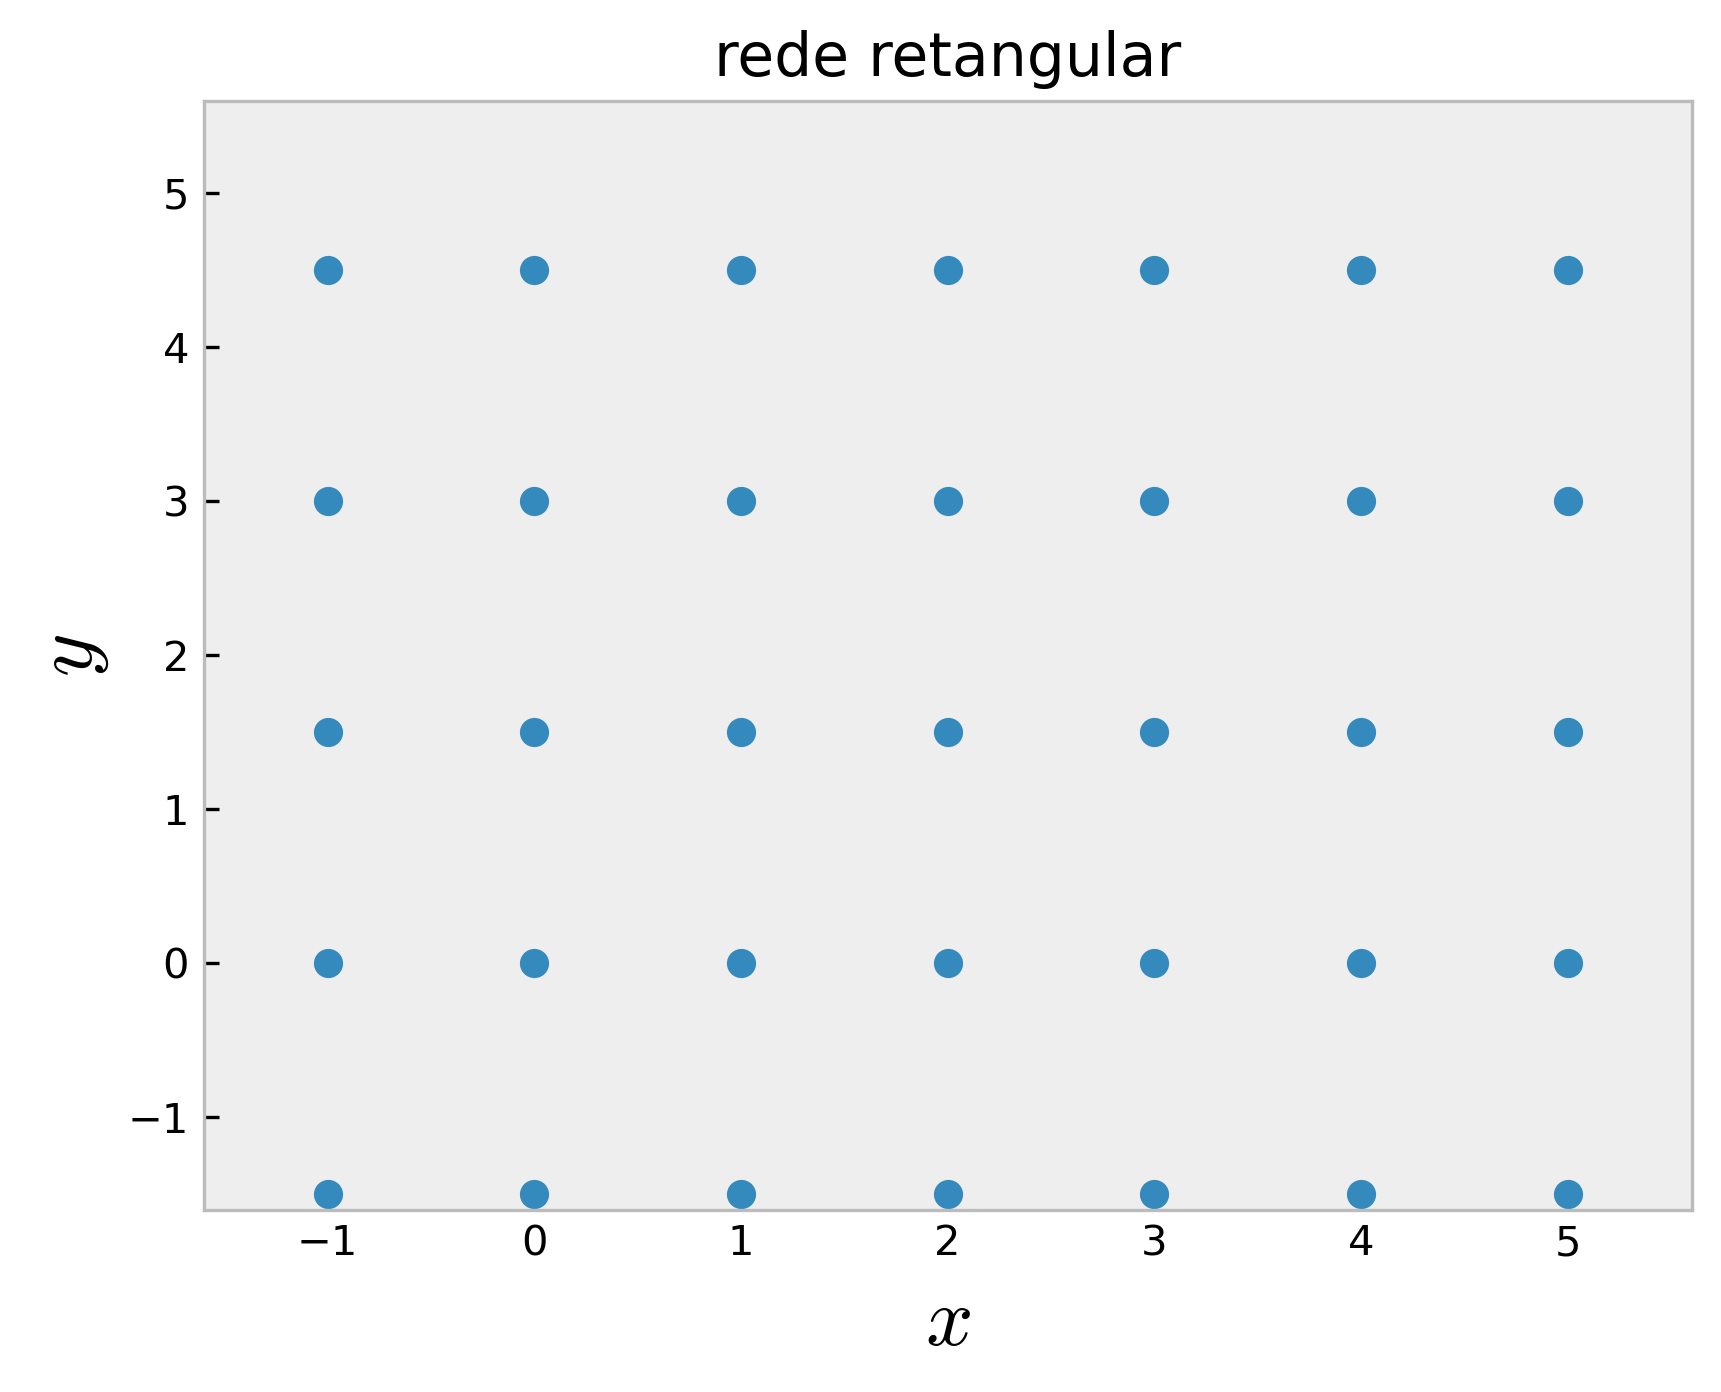
\includegraphics[width=0.35\linewidth]{fig/lattice_retang.png}
\caption{Rede Retangular.}
\label{fig:lat-retang}
\end{figure}
\item Rede hexagonal: pode-se achar dois vetores primitivos que formam um ângulo de $60^\circ$ entre si e tenham o mesmo módulo. Exemplo: $\a_1 = a \vu{x}$ e $\a_2 = a \qty(\frac{1}{2} \vu{x} + \frac{\sqrt{3}}{2} \vu{y})$.
\begin{figure}[H]
\centering
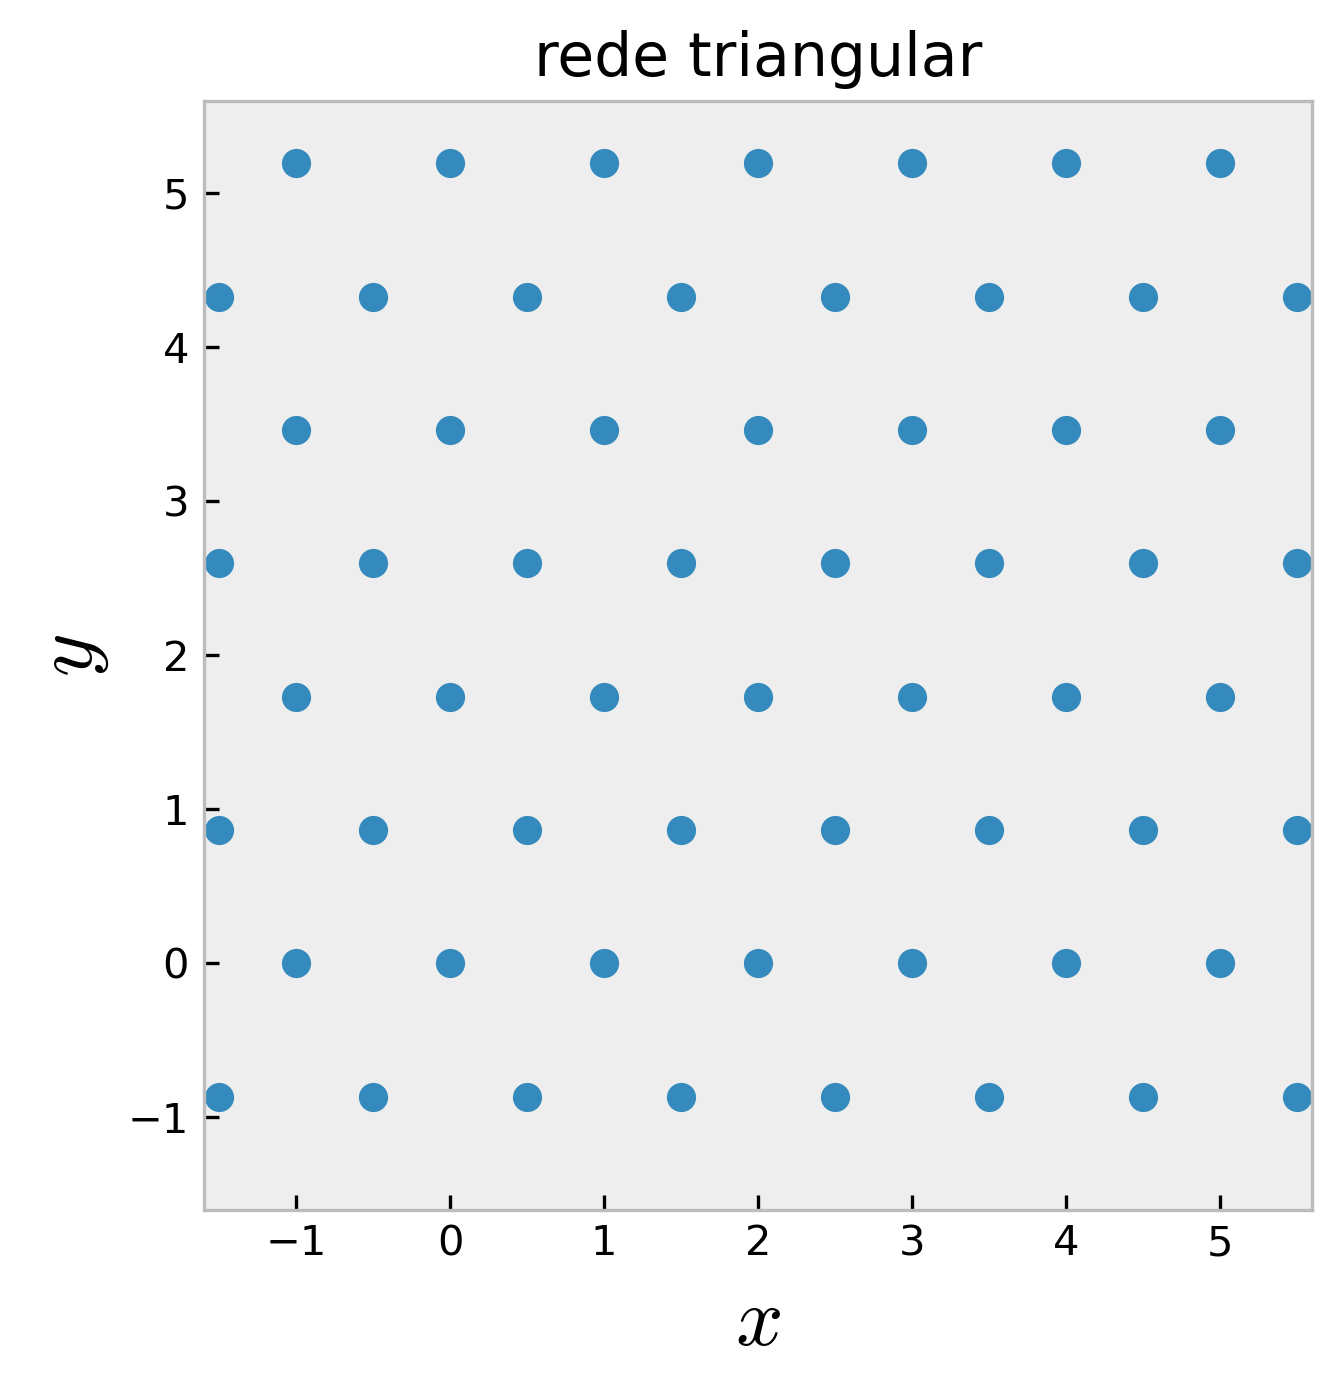
\includegraphics[width=0.35\linewidth]{fig/lattice_triang.png}
\caption{Rede Hexagonal (Triangular).}
\label{fig:lat-triang}
\end{figure}
\item Rede oblíqua: pode-se achar dois vetores primitivos que formam um ângulo \textbf{diferente} de $90^\circ$ e que tenham \textbf{módulos diferentes}. Exemplo: $\a_1 = a \vu{x}$ e $\a_2 = a (0.3 \vu{x} + 0.9\vu{y})$.
\begin{figure}[H]
\centering
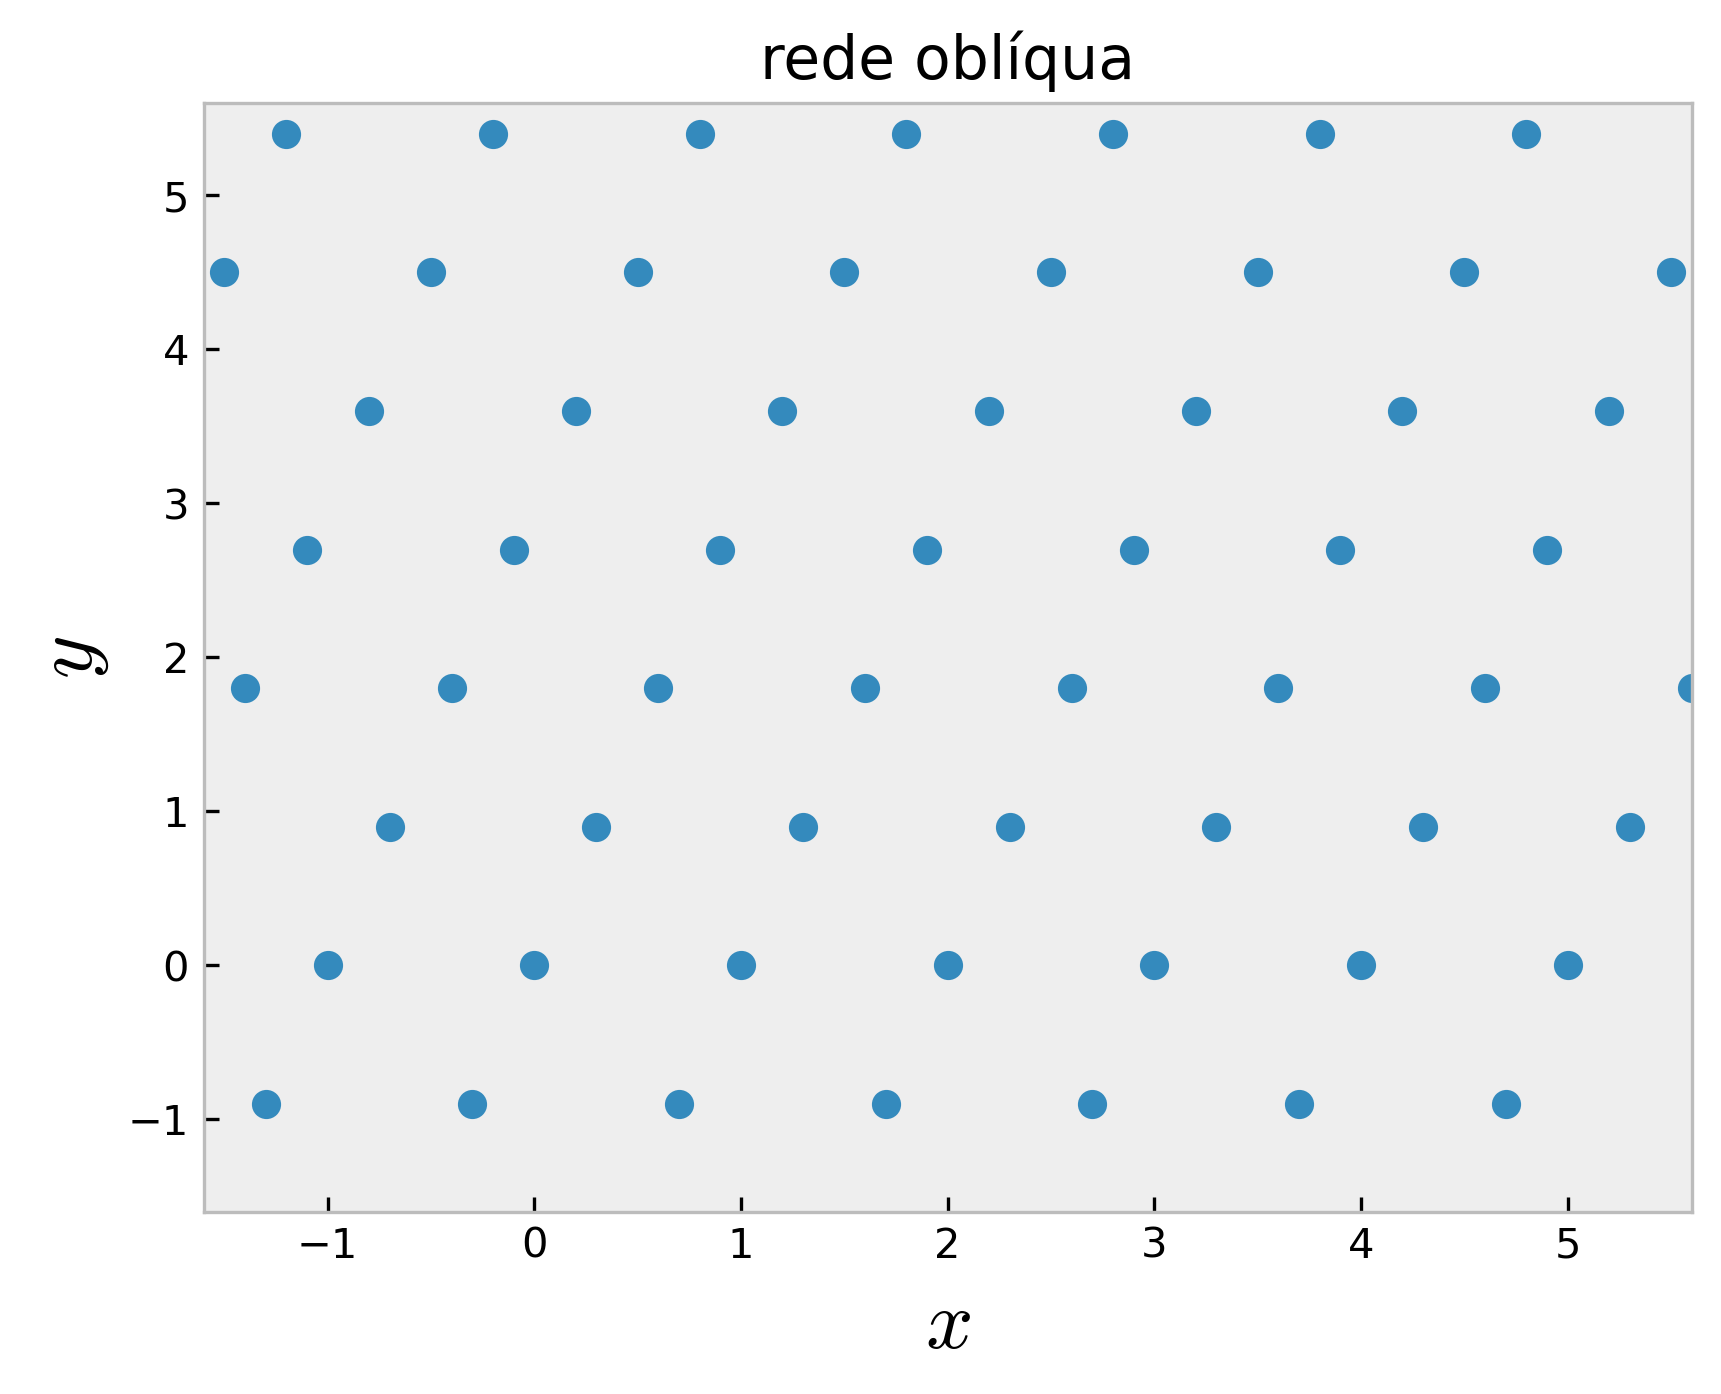
\includegraphics[width=0.35\linewidth]{fig/lattice_obliq.png}
\caption{Rede Oblíqua.}
\label{fig:lat-obliq}
\end{figure}
\end{itemize}

\n

(c) A rede hexagonal tem o grupo de simetria diedral $D_6$, que é composto de 12 elementos distintos. Esse grupo é gerado somente através de duas operações, uma rotação $\rho$ de $60^\circ$ e uma reflexão $\sigma$ qualquer. Assim, todos as operações de simetria são dados por $D_6 = \{1, \rho, \rho^2, \rho^3, \rho^4, \rho^5, \s, \rho\s, \rho^2\s, \rho^3\s, \rho^4\s, \rho^5\s\}$. Esses elementos são algum dos seguintes:
\begin{itemize}
\item Rotações de $60^\circ$: 6 elementos contando com a identidade ($0^\circ$, $60^\circ$, $120^\circ$, $180^\circ$, $240^\circ$, $300^\circ$).
\item Reflexões em alguns dos seguintes 6 eixos: três por \textcolor{red}{eixos que ligam vértices do hexágono} e três por \textcolor{blue}{eixos que passam pelo meio de arestas do hexágono}.
\begin{figure}[H]
\centering
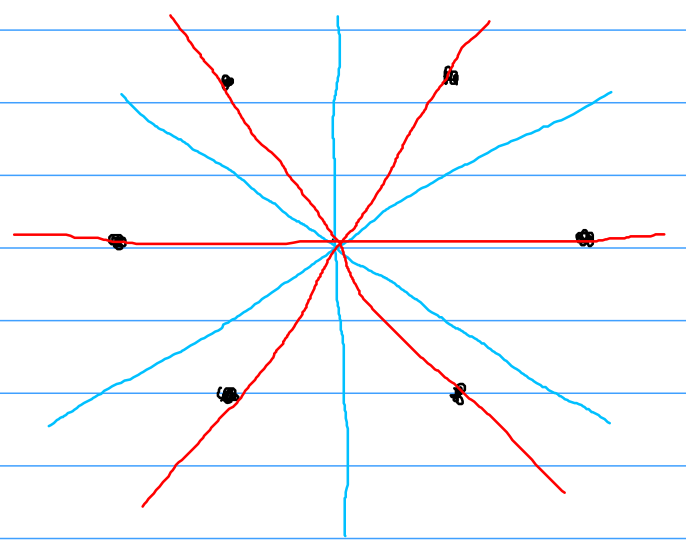
\includegraphics[width=0.5\linewidth]{fig/hex_reflex.png}
\caption{Seis eixos de reflexão da rede hexagonal.}
\label{fig:hex_reflex}
\end{figure}
\item Inversão: que pode ser vista como uma rotação de $180^\circ$.
\end{itemize}

(d) Não tenho certeza o que você quer dizer com rede ``oblíqua triangular'', mas acredito que seria com dois vetores primitivos $\a_1$ e $\a_2$ formando $60^\circ$ entre si mas com módulos diferentes. Por exemplo, $\a_1 = a \vu{x}$ e $\a_2 = 1.3 a \qty(\frac{1}{2} \vu{x} + \frac{\sqrt{3}}{2} \vu{y})$. \textbf{NÃO TENHO CERTEZA.}

\n

(e) Podemos chegar à estrutura do grafeno a partir da rede hexagonal com vetores de rede $\a_1 = a \vb{x}$ e $\a_2 = a \qty(\frac{1}{2} \vu{x} + \frac{\sqrt{3}}{2} \vu{y})$ e dois vetores compondo a base (os dois átomos de carbono inequivalentes da célula unitária do grafeno), sendo eles $\r_1 = \0$ e $\r_2 = a \qty(\frac{1}{2}\vu{x} + \frac{\sqrt{3}}{3}\vb{y})$.
\begin{figure}[H]
\centering
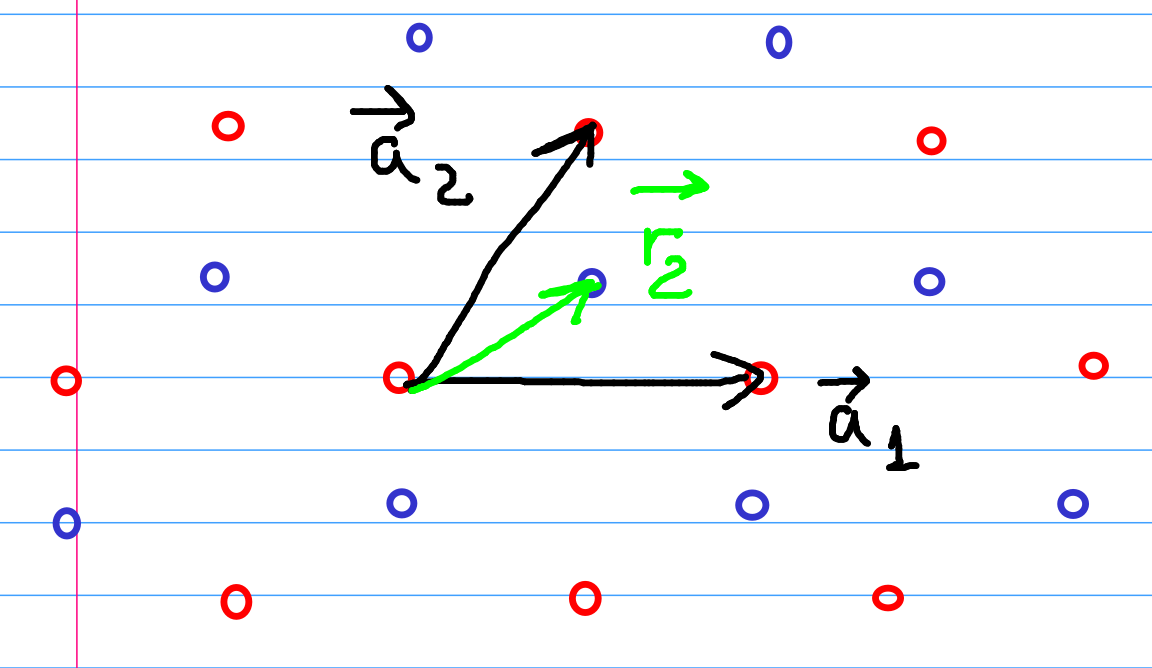
\includegraphics[width=0.4\linewidth]{fig/graphene_vec}
\caption{Estrutura do grafeno e vetores.}
\label{fig:graphene_vec}
\end{figure}

\section{}

(a) Quadrada 2D:
\begin{figure}[H]
\centering
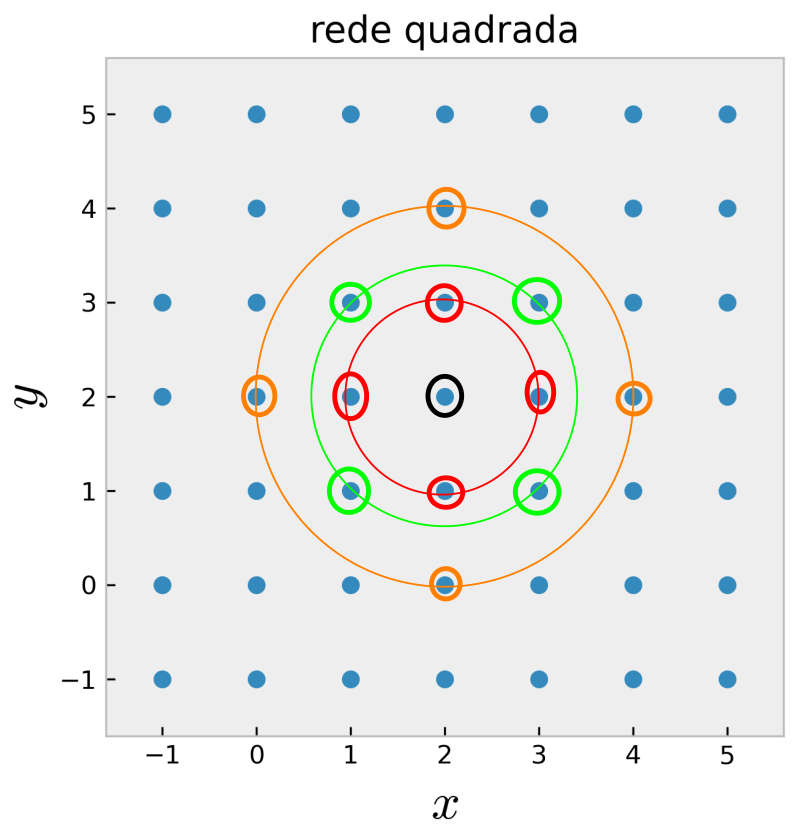
\includegraphics[width=0.3\linewidth]{fig/nn_quad}
\caption{Primeiros, segundos e terceiros vizinhos na rede quadrada.}
\label{fig:nn_quad}
\end{figure}
\begin{itemize}
\item 4 primeiros vizinhos com distância $a$.
\item 4 segundos vizinhos com distância $a\sqrt{2}$.
\item 4 terceiros vizinhos com distância $2a$.
\end{itemize}

(b) Hexagonal 2D:
\begin{figure}[H]
\centering
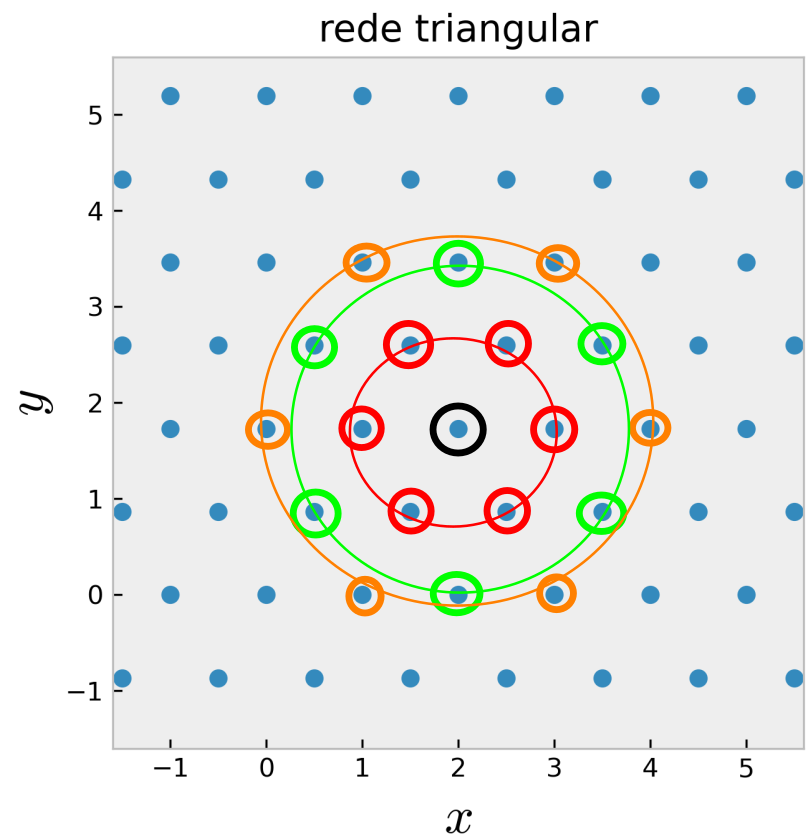
\includegraphics[width=0.3\linewidth]{fig/nn_triang}
\caption{Primeiros, segundos e terceiros vizinhos na rede hexagonal.}
\label{fig:nn_triang}
\end{figure}
\begin{itemize}
\item 6 primeiros vizinhos com distância $a$.
\item 6 segundos vizinhos com distância $a\sqrt{3}$.
\item 6 terceiros vizinhos com distância $2a$.
\end{itemize}

Para as estruturas 3D eu não vou desenhar, mas é fácil contar os vizinhos por combinatória $\sqrt{(\;)^2+(\;)^2+(\;)^2}$.

\n

(c) Cúbica:

\begin{itemize}
\item 6 primeiros vizinhos com distância $a$.
\item 12 segundos vizinhos com distância $a\sqrt{2}$.
\item 8 terceiros vizinhos com distância $a\sqrt{3}$.
\end{itemize}

(d) Cúbica de Corpo Centrado: ($a$ a distância dos vetores primitivos na célula convencional do bcc)

\begin{itemize}
\item 8 primeiros vizinhos com distância $a \frac{\sqrt{3}}{2}$.
\item 6 segundos vizinhos com distância $a$.
\item 12 terceiros vizinhos com distância $a\sqrt{2}$.
\end{itemize}



\end{document}
